\chapter{Workloads}
\label{ch:workloads}

In order to evaluate the effectiveness of CRAFTS methods, we developed a series of data sets. The methods by which each of these workloads were generated as well as any interesting features they posses are outlined below.

As a real-world test, we used the Wikipedia HTTP trace logs published by the WikiBench researchers \cite{wikitraces}. These logs detailed access to Wikipedia for a two month period spanning September and October of 2007. The format of these logs detailed a single request per line and included a timestamp and request url. Since CRAFTS requires input to be given in aggregate, it was necessary to transform the data into the appropriate format. Additionally, the size of the logs was large enough (almost 1TB) the we decided to use Hadoop to consolidate the request data into five-minute request per second averages. Pseudocode for our MapReduce job can be seen below.

\begin{algorithm}[H]
\KwData{$line =$ A line from the input request logs}
\Begin{
    $time =$ Extract time from $line$\;
    
    $emit(time, 1)$\;
}
\caption{WikiBench transformation map function}
\end{algorithm}

\begin{algorithm}[H]
\KwData{$time =$ A time emitted by the $map$ function \\
        $values =$ All of the values emmited with the given $time$}
\Begin{
    $emit(time, sum(values))$\;
}
\caption{WikiBench transformation reduce job}
\end{algorithm}

The temporal data generated as a result of our MapReduce job can be seen in \Cref{fig:wikibench2}. This data shows clear diurnal periodicity, as well as a weekly modulation.

\begin{figure}
\centering
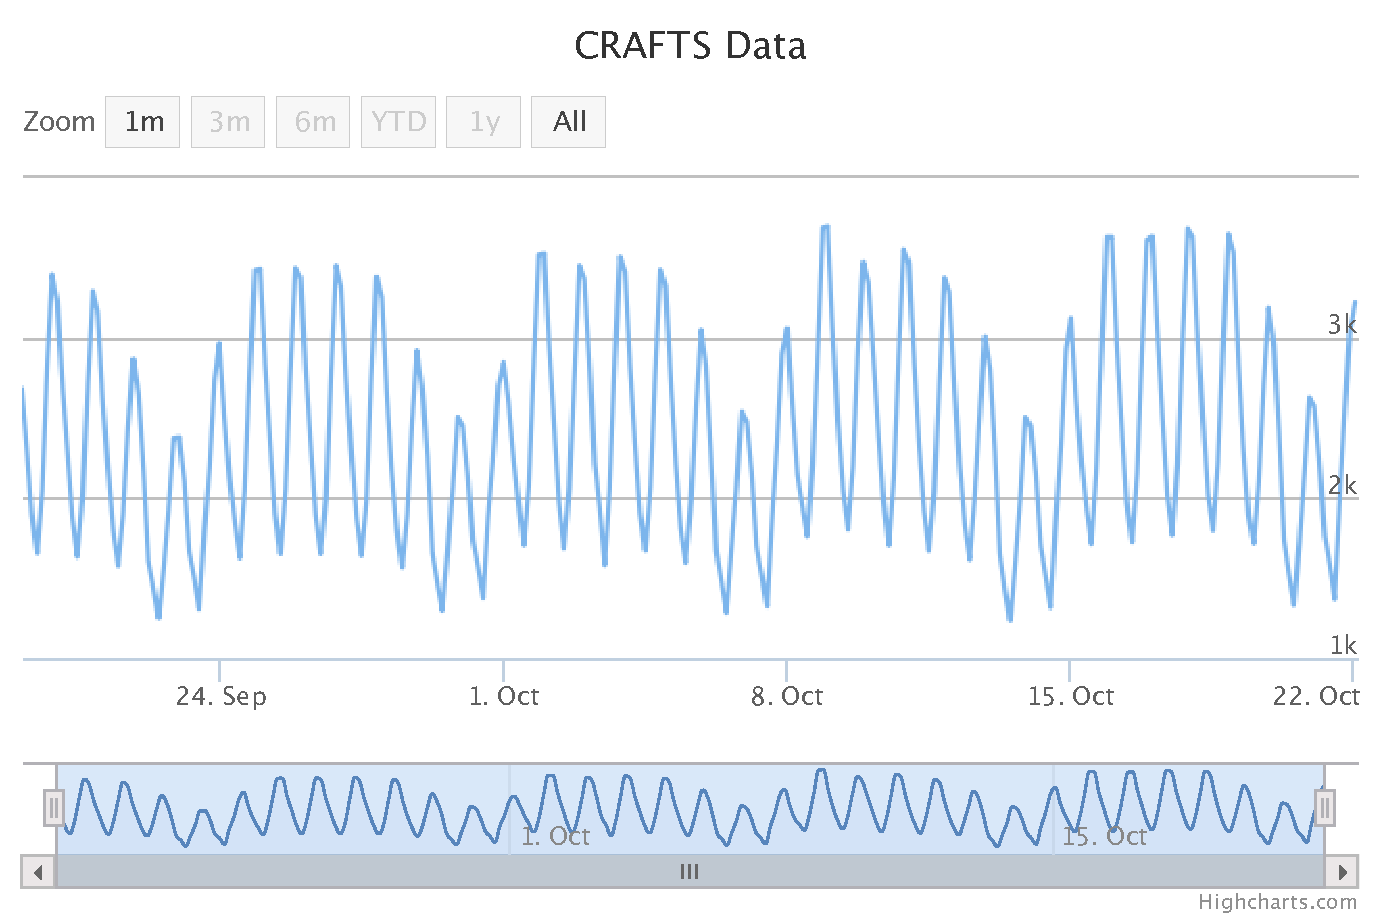
\includegraphics[width=\textwidth]{charts/wikibench.pdf}
\caption{A time-series plot of Wikipedia input data.}
\label{fig:wikibench2}
\end{figure}

This raw Wikipedia workload serves as the baseline for our evaluation. In order to see how our prediction methods are affected by anomalies in the monitoring data, we generated four additional workloads using ARTS' events feature. These workloads introduce outages and usage spikes into the third and fourth weeks of the workload. The third and fourth weeks were chosen because they will be in the training window and prediction horizon, respectively, for our evaluation trials. \Cref{tab:workloads} shows the exact parameters used to generate these workloads and the names by which they will be referred to.

It is important to note that we only use the term ``horizon'' for simplicity. As described in \Cref{ch:policies}, some of our predictors make only short-term predictions, predicting only one point at a time. Anomalies which are present in the ``prediction horizon'' will end up being a part of their training data once the predictor is looking past that point in time.

\begin{table}
\centering
\begin{tabular}{| l | l | l | l | l |}
\hline
Name & Anomaly Type & Start & End & Magnitude \\ \hline
Baseline & none & & & \\ \hline
Training outage & outage & 2007-10-12T17:00 & 2007-10-12T18:00 & \\ \hline
Horizon outage & outage & 2007-10-19T17:00 & 2007-10-19T18:00 & \\ \hline
Training spike & spike & 2007-10-12T17:00 & 2007-10-12T17:15 & 2.0 \\ \hline
Horizon spike & spike & 2007-10-19T17:00 & 2007-10-19T17:15 & 2.0 \\ \hline
\end{tabular}
\caption{ARTS parameters and titles of our evaluation workloads}
\label{tab:workloads}
\end{table}